\section{Variable-density results}
\label{sec:variable_density}
\citet{khorasani-szekely-ascher-2015}

\subsection{Linearized operator at zero horizontal wavenumber}

For completeness, we record the form taken by the variable-density linearized
operator for a perturbation that is uniform in the horizontal plane. Setting
\(k=0\) gives \(\nabla_{xy}^{2}=0\) and \(\nabla^{2}=\partial_{zz}\). It is
convenient to introduce the corresponding one-dimensional divergence operators
\begin{equation}
  \mathscr{L}_{\rho}^{(0)}(\star)
  =-\Sch^{-1}\partial_{zz}\!\left(\frac{\star}{\rho_0}\right),
  \qquad
  \dot{\mathscr{L}}_{\rho}^{(0)}(\star)
  =-\Sch^{-1}\partial_{zz}\!\left[
    \frac{\partial}{\partial t}\left(\frac{\star}{\rho_0}\right)
  \right].
  \label{eq:vd_k0_divergence_operators}
\end{equation}
The operator blocks defined in \cref{eq:A_B_operators} then reduce to
\begin{subequations}
\label{eq:vd_k0_operators}
\begin{align}
  \widehat{\mathscr{B}}_{ww}^{(0)}
  &= -\left(\rho_0'\partial_z+\rho_0\partial_{zz}\right), \\
  \widehat{\mathscr{B}}_{w\rho}^{(0)}
  &= \left(\rho_0'+\rho_0\partial_z\right)
     \mathscr{L}_{\rho}^{(0)}, \\
  \widehat{\mathscr{A}}_{ww}^{(0)}
  &= -\mu_0\partial_{zzzz}-2\mu_0'\partial_{zzz}
     -\mu_0''\partial_{zz}, \\
  \widehat{\mathscr{A}}_{w_0w}^{(0)}
  &= \rho_0w_0\partial_{zzz}+(\rho_0w_0)'\partial_{zz}, \\
  \widehat{\mathscr{A}}_{w\rho}^{(0)}
  &= \left(\mu_0\partial_{zzz}+2\mu_0'\partial_{zz}
     +\mu_0''\partial_z\right)\mathscr{L}_{\rho}^{(0)}, \\
  \widehat{\mathscr{A}}_{w_0\rho}^{(0)}
  &= -\left((\rho_0w_0)'\partial_z+\rho_0w_0\partial_{zz}\right)
     \mathscr{L}_{\rho}^{(0)}
     -\left(\rho_0'+\rho_0\partial_z\right)
     \dot{\mathscr{L}}_{\rho}^{(0)}, \\
  \widehat{\mathscr{A}}_{\rho w}^{(0)}
  &= -\rho_0', \\
  \widehat{\mathscr{A}}_{\rho\rho}^{(0)}
  &= -\left(w_0\partial_z+w_0'\right)
     -\rho_0\mathscr{L}_{\rho}^{(0)}.
\end{align}
\end{subequations}
The two divergence operators can now be expanded explicitly as
\begin{equation}
  \mathscr{L}_{\rho}^{(0)}(\rho)
  =-\Sch^{-1}\partial_{zz}\!\left(\frac{\rho}{\rho_0}\right),
  \qquad
  \dot{\mathscr{L}}_{\rho}^{(0)}(\rho)
  =\Sch^{-1}\partial_{zz}\!\left(
    \frac{\rho\,\partial_t\rho_0}{\rho_0^2}
  \right),
  \label{eq:vd_k0_expanded_divergence_operators}
\end{equation}
where the overdot differentiates the time-dependent operator while holding its
argument fixed. Hence
\begin{equation}
  \partial_t\!\left[\mathscr{L}_{\rho}^{(0)}(\rho)\right]
  =\mathscr{L}_{\rho}^{(0)}(\partial_t\rho)
   +\dot{\mathscr{L}}_{\rho}^{(0)}(\rho).
  \label{eq:vd_k0_operator_product_rule}
\end{equation}

At zero horizontal wavenumber, the divergence constraint itself becomes
\begin{equation}
  \partial_z w
  =-\Sch^{-1}\partial_{zz}\!\left(\frac{\rho}{\rho_0}\right).
  \label{eq:vd_k0_divergence_constraint}
\end{equation}
Using this constraint and its time derivative in the vertical-velocity equation
makes all of its terms cancel. For example, its remaining spatial terms are
\begin{equation}
  \partial_z\!\left(\mu_0\partial_{zz}w\right)
  -\rho_0w_0\partial_{zz}w
  -\left(\mu_0\partial_{zz}+\mu_0'\partial_z
  -\rho_0w_0\partial_z\right)
  \mathscr{L}_{\rho}^{(0)}(\rho)=0,
\end{equation}
because \(\partial_z w=\mathscr{L}_{\rho}^{(0)}(\rho)\). Thus, at \(k=0\),
the pressure-eliminated vertical-momentum equation supplies no additional
dynamics.

Integrating \eqref{eq:vd_k0_divergence_constraint} once and applying the
far-field conditions gives
\begin{subequations}
  \label{eq:vd_k0_linearized_system}
  \begin{align}
    w
    &=-\Sch^{-1}\partial_z\!\left(\frac{\rho}{\rho_0}\right),
    \label{eq:vd_k0_vertical_velocity}\\
    \partial_t\rho+\partial_z(w_0\rho)
    &=\Sch^{-1}\partial_z\!\left[
      \rho_0\partial_z\!\left(\frac{\rho}{\rho_0}\right)
    \right].
    \label{eq:vd_k0_density}
  \end{align}
\end{subequations}
The \(k=0\) problem therefore reduces to a single scalar equation for \(\rho\),
after which \(w\) follows directly from \eqref{eq:vd_k0_vertical_velocity}.

To examine its modal behaviour, freeze the base state at a time \(t_0\) and set
\(\rho(z,t)=\phi(z)e^{\sigma t}\). The eigenvalue problem is simply
\begin{equation}
  \sigma\phi
  =-\partial_z(w_0\phi)
  +\Sch^{-1}\partial_z\!\left[
    \rho_0\partial_z\!\left(\frac{\phi}{\rho_0}\right)
  \right].
  \label{eq:vd_k0_eigenvalue_problem}
\end{equation}
This is a conservative one-dimensional advection--diffusion operator and hence
has no eigenvalues with positive real part. In the uniform far field,
\(w_0\to0\) and \(\rho_0\) is constant, so a vertical Fourier mode
\(\phi\sim e^{\mathrm{i}mz}\) has the growth rate
\begin{equation}
  \sigma(m)=-\frac{m^2}{\Sch}\leq0.
  \label{eq:vd_k0_growth_rate}
\end{equation}
Thus, on an unbounded domain, the spectral bound is \(\sigma_{\max}=0\), reached
in the limit \(m\to0\); every finite vertical wavenumber decays. On a finite
domain the largest eigenvalue is strictly negative and depends on the vertical
boundary conditions.

Expanding the diffusive flux in \eqref{eq:vd_k0_density} writes the same
equation in conservative advection--diffusion form,
\begin{equation}
  \partial_t\rho
  =
  \Sch^{-1}\partial_{zz}\rho
  -
  \partial_z\!\left[
    \left(w_0+\Sch^{-1}\left(\ln\rho_0\right)'\right)\rho
  \right],
  \label{eq:vd_k0_conservative_form}
\end{equation}
or, equivalently, as an advection--reaction--diffusion equation
\(\partial_t\rho=a\,\partial_{zz}\rho-c\,\partial_z\rho+r\,\rho\) with
\begin{subequations}
  \label{eq:vd_k0_ard_coefficients}
  \begin{align}
    a &= \Sch^{-1},
    \label{eq:vd_k0_ard_a}\\
    c &= w_0+\Sch^{-1}\frac{\rho_0'}{\rho_0},
    \label{eq:vd_k0_ard_c}\\
    r &= -\left[w_0'+\Sch^{-1}\left(\ln\rho_0\right)''\right]=-c',
    \label{eq:vd_k0_ard_r}
  \end{align}
\end{subequations}
where \(\left(\ln\rho_0\right)''=\rho_0''/\rho_0-\left(\rho_0'/\rho_0\right)^2\).
The reaction coefficient is minus the derivative of the advection coefficient,
which is the conservative structure already used above. The base state
\eqref{eq:vd_base_state_w0} gives \(w_0=\rho_0'/\rho_0=\left(\ln\rho_0\right)'\),
so that
\begin{equation}
  \partial_t\rho
  =
  \Sch^{-1}\partial_{zz}\rho
  -
  \left(1+\Sch^{-1}\right)\partial_z\!\left(w_0\rho\right),
  \qquad
  c=\left(1+\Sch^{-1}\right)w_0,
  \qquad
  r=-\left(1+\Sch^{-1}\right)w_0' ,
  \label{eq:vd_k0_ard_base_state}
\end{equation}
and, with \(w_0'=-2zw_0/\delta^{2}-w_0^{2}\),
\(r=\left(1+\Sch^{-1}\right)w_0\left(2z/\delta^{2}+w_0\right)\).

%k-star and sigma-star grids at delta0 = 2: rows sweep Sc and columns sweep At,
%So a row shares one ordinate scale set by its leftmost panel. Panels are
%Generated by codes/4_VD/P2_sigma_kstar.m.
\newcommand{\VDStarGrid}[2]{%
\begin{figure}[p]
  \centering
  \begin{minipage}[t]{0.24\textwidth}\centering
    \tikzfig{#1_VD_Sc_0p25_d0_2_At_0p05}
  \end{minipage}\hfill
  \begin{minipage}[t]{0.24\textwidth}\centering
    \tikzfig{#1_VD_Sc_0p25_d0_2_At_0p2}
  \end{minipage}\hfill
  \begin{minipage}[t]{0.24\textwidth}\centering
    \tikzfig{#1_VD_Sc_0p25_d0_2_At_0p5}
  \end{minipage}\hfill
  \begin{minipage}[t]{0.24\textwidth}\centering
    \tikzfig{#1_VD_Sc_0p25_d0_2_At_0p7}
  \end{minipage}
  \\[2pt]
  \begin{minipage}[t]{0.24\textwidth}\centering
    \tikzfig{#1_VD_Sc_1_d0_2_At_0p05}
  \end{minipage}\hfill
  \begin{minipage}[t]{0.24\textwidth}\centering
    \tikzfig{#1_VD_Sc_1_d0_2_At_0p2}
  \end{minipage}\hfill
  \begin{minipage}[t]{0.24\textwidth}\centering
    \tikzfig{#1_VD_Sc_1_d0_2_At_0p5}
  \end{minipage}\hfill
  \begin{minipage}[t]{0.24\textwidth}\centering
    \tikzfig{#1_VD_Sc_1_d0_2_At_0p7}
  \end{minipage}
  \\[2pt]
  \begin{minipage}[t]{0.24\textwidth}\centering
    \tikzfig{#1_VD_Sc_10_d0_2_At_0p05}
  \end{minipage}\hfill
  \begin{minipage}[t]{0.24\textwidth}\centering
    \tikzfig{#1_VD_Sc_10_d0_2_At_0p2}
  \end{minipage}\hfill
  \begin{minipage}[t]{0.24\textwidth}\centering
    \tikzfig{#1_VD_Sc_10_d0_2_At_0p5}
  \end{minipage}\hfill
  \begin{minipage}[t]{0.24\textwidth}\centering
    \tikzfig{#1_VD_Sc_10_d0_2_At_0p7}
  \end{minipage}
  \caption{#2 in the variable-density regime at \(\delta_0=2\), as defined
  in~\eqref{eq:maximum_growth_definitions}. Rows correspond to \(\Sch=0.25\),
  \(1\), and \(10\); columns correspond to \(\Atw=0.05\), \(0.2\), \(0.5\), and
  \(0.7\), as labelled above each panel. Each panel compares the three viscosity
  contrasts \(\Amu=-0.9\), \(0\), and \(0.9\). The ordinate range and the time
  window are shared along each row, since both change strongly with \(\Sch\) and
  weakly with \(\Atw\).}
  \label{fig:VD_#1_grid}
\end{figure}%
}

\VDStarGrid{sigmastar}{Maximum mean growth rate \(\overline{\sigma}_\ast(t)\)}


% Three-dimensional growth-rate grids at delta0 = 2, one figure per viscosity
% contrast: rows sweep Sc and columns sweep At. Panels are generated by
% codes/4_VD/P3_growth_3D.m.
\newcommand{\VDThreeDGrid}[2]{%
\begin{figure}[p]
  \centering
  \begin{minipage}[t]{0.24\textwidth}\centering
    \tikzfig{sigma3D_VD_Sc_0p25_d0_2_At_0p05_Amu_#1}
  \end{minipage}\hfill
  \begin{minipage}[t]{0.24\textwidth}\centering
    \tikzfig{sigma3D_VD_Sc_0p25_d0_2_At_0p2_Amu_#1}
  \end{minipage}\hfill
  \begin{minipage}[t]{0.24\textwidth}\centering
    \tikzfig{sigma3D_VD_Sc_0p25_d0_2_At_0p5_Amu_#1}
  \end{minipage}\hfill
  \begin{minipage}[t]{0.24\textwidth}\centering
    \tikzfig{sigma3D_VD_Sc_0p25_d0_2_At_0p7_Amu_#1}
  \end{minipage}
  \\[2pt]
  \begin{minipage}[t]{0.24\textwidth}\centering
    \tikzfig{sigma3D_VD_Sc_1_d0_2_At_0p05_Amu_#1}
  \end{minipage}\hfill
  \begin{minipage}[t]{0.24\textwidth}\centering
    \tikzfig{sigma3D_VD_Sc_1_d0_2_At_0p2_Amu_#1}
  \end{minipage}\hfill
  \begin{minipage}[t]{0.24\textwidth}\centering
    \tikzfig{sigma3D_VD_Sc_1_d0_2_At_0p5_Amu_#1}
  \end{minipage}\hfill
  \begin{minipage}[t]{0.24\textwidth}\centering
    \tikzfig{sigma3D_VD_Sc_1_d0_2_At_0p7_Amu_#1}
  \end{minipage}
  \\[2pt]
  \begin{minipage}[t]{0.24\textwidth}\centering
    \tikzfig{sigma3D_VD_Sc_10_d0_2_At_0p05_Amu_#1}
  \end{minipage}\hfill
  \begin{minipage}[t]{0.24\textwidth}\centering
    \tikzfig{sigma3D_VD_Sc_10_d0_2_At_0p2_Amu_#1}
  \end{minipage}\hfill
  \begin{minipage}[t]{0.24\textwidth}\centering
    \tikzfig{sigma3D_VD_Sc_10_d0_2_At_0p5_Amu_#1}
  \end{minipage}\hfill
  \begin{minipage}[t]{0.24\textwidth}\centering
    \tikzfig{sigma3D_VD_Sc_10_d0_2_At_0p7_Amu_#1}
  \end{minipage}
  \\[2pt]
  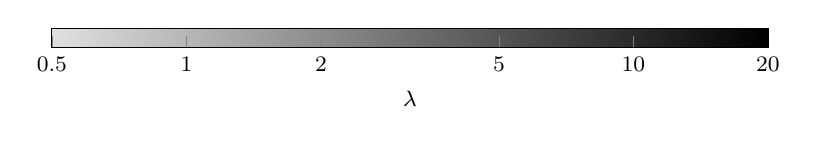
\begin{tikzpicture}
\begin{axis}[
hide axis, scale only axis,
width=0.75\textwidth, height=0pt,
colormap={sigmamap}{rgb(0.0000)=(0.8800,0.8800,0.8800); rgb(0.1000)=(0.7903,0.7903,0.7903); rgb(0.2000)=(0.7040,0.7040,0.7040); rgb(0.3000)=(0.6143,0.6143,0.6143); rgb(0.4000)=(0.5280,0.5280,0.5280); rgb(0.5000)=(0.4383,0.4383,0.4383); rgb(0.6000)=(0.3520,0.3520,0.3520); rgb(0.7000)=(0.2623,0.2623,0.2623); rgb(0.8000)=(0.1760,0.1760,0.1760); rgb(0.9000)=(0.0863,0.0863,0.0863); rgb(1.0000)=(0.0000,0.0000,0.0000)},
point meta min=-0.30103, point meta max=1.30103,
colorbar horizontal,
colorbar style={
  width=0.75\textwidth, height=7pt,
  at={(0,0)}, anchor=north west,
  xlabel={$\lambda$},
  xlabel style={font=\footnotesize},
  tick label style={font=\footnotesize},
  xtick pos=bottom,
  xtick={-0.30103,0,0.30103,0.69897,1,1.30103},
  xticklabels={0.5,1,2,5,10,20},
},
]
\addplot[draw=none] coordinates {(0,0)};
\end{axis}
\end{tikzpicture}

  \caption{Three-dimensional mean growth rate \(\overline{\sigma}_{3D}(t)\) in
  the variable-density regime at \(\Amu=#2\) and \(\delta_0=2\). Rows
  correspond to \(\Sch=0.25\), \(1\), and \(10\); columns correspond to
  \(\Atw=0.05\), \(0.2\), \(0.5\), and \(0.7\), as labelled above each panel.
  Each panel contains 20 logarithmically spaced integral correlation lengths
  \(0.5\leq\lambda\leq20\), progressing from light gray to black as \(\lambda\)
  increases, and the (\dashlegend) line marks neutral growth. The ordinate range
  is shared along each row.}
  \label{fig:VD_sigma3D_grid_Amu#1}
\end{figure}%
}

\VDThreeDGrid{m0p9}{-0.9}
\VDThreeDGrid{0}{0}
\VDThreeDGrid{0p9}{0.9}
